% diagrams/lineas-espiral.tex -- una espiral y una línea suelta, para
% "Completa": un caracol, una piruleta, la cola de un dragón, un
% remolino de viento, una rosa vista desde arriba...
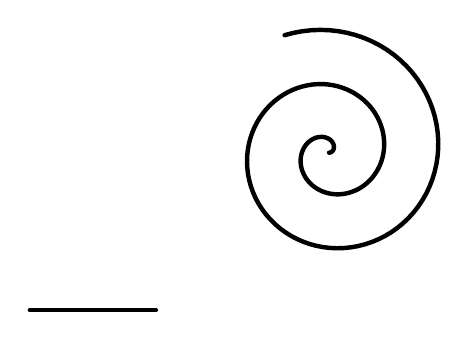
\begin{tikzpicture}[line width=1.6pt, line cap=round, line join=round]
  \draw[domain=0:14.5, samples=200, variable=\t]
    plot ({0.11*\t*cos(\t r)}, {0.11*\t*sin(\t r) - 0.6});
  \draw (-3.8,-2.6) -- (-2.2,-2.6);
\end{tikzpicture}
